\chapter{Bayesian Inference}

With the theoretical and practical aspects of probability
theory at our disposal, we are finally ready to formally define 
concepts like measurement, inference, and decision making.  
Here we consider a Bayesian approach to these ideas, although
the same foundation is also critical for constructing a rigorous
frequentist approach to inference as well.

\section{Modeling Measurements}

We begin by defining measurements before considering how
to model that measurements mathematically.

\subsection{The Data Generating Process}

The basic assumption underlying inference is that there is some
observable process that we would like to understand, or at least
some latent process that has observable consequences.

These observable consequences manifest as logical statements,
but in practice we can observe only variable measurements
of those statements.  In order to formalize these concepts we
assume that this variability is sufficiently well-behaved that we
can model it with probability theory.  More formally, we assume
that the process under consideration defines a probability 
distribution, $\PP_{D}$ over some measurement space, $D$, 
with measurements defined as events in the corresponding
event space.  

Although we have assumed the existence of a \emph{data
generating process}, $\PP_{D}$, we have intentionally not
assumed any philosophical interpretation of it.  In particular, we
are indifferent to the ultimate source of the variability in the
measurements quantified by $\PP_{D}$: it could be some
ontological variability inherent to the system or just some
epistemological variability due to our ignorance of the underlying 
system.  The only assumption we have made is that the
measurements are repeatable and variable, and that this
variability is sufficiently well-behaved to be quantified by
probability theory. 

We can assume the existence of a data generating process, 
but we don't know anything about it until we start making 
measurements.  An infinite number of measurements would 
certainly inform us of the data generating process exactly,
but measurements are expensive and in practice we have
to learn about the data generating process from only a few
measurements, if not just a single measurement. \emph{Inference}
is the process of learning about the data generating process
using only a finite number measurements.  

\subsection{Big Worlds and Small Worlds}

If we want to learn about the data generating process we have
to consider all possible data generating process we could
encounter or, equivalently, all possible probability distributions
over the sample space, $D$.  We refer to this massive set, 
$\mathcal{P}_{D}$ as the \emph{the big world} (Figure \ref{fig:big_world}).  

\begin{figure*}
\centering
\begin{tikzpicture}[scale=0.40, thick]

  \draw[color=white] (-15, 0) -- (15, 0);

  \fill[mid] (0, 0) ellipse (13 and 7);
  \node at (12, -6) {$\mathcal{P}_{D}$};
  
  \fill[color=white] (-7, 3) circle (4pt)
  node[right, color=white] {$\PP_{D}$};
  
\end{tikzpicture}
\caption{Once we have defined a measurement space, $D$, the latent data
generating process, $\PP_{D}$, must be contained in the space of all 
possible data generating processes over $D$, $\mathcal{P}_{D}$.
}
\label{fig:big_world}
\end{figure*}

The big world is much too ungainly to be even well-defined in 
practice, let alone exhaustively explored.  Instead we have to limit 
our consideration to only a subset of probability distributions over 
the measurement space called a \emph{small world}, $\Theta \subset
\mathcal{P}_{D}$ (Figure \ref{fig:small_worlds}a).  An expression
of the small world is called a \emph{parameterization} of our model.

Each point in the small world, $\theta \in \Theta$, identifies a unique 
probability distribution over data.  Consequently the small world defines 
a collection of probability distribution over the measurement space,
%
\begin{align*}
\mathbb{L}
&: \EV{D} \times \Theta \rightarrow \left[0, 1 \right] \\
&\quad \left( E_{D}, \theta \right) \;\; \mapsto 
\mathbb{L} \! \left[ E_{D} \mid \theta \right].
\end{align*}
%
known as the \emph{likelihood}.  We can also interpret the likelihood
as a conditional probability distribution over implications from our
small world model to the measurement space.

Regardless of how it is chosen, the assumption of any specific 
small world can have drastic limitations on inference.  Because any
small world is only a shallow approximation of reality, for example, 
it is unlikely to contain the latent data generating process (Figure
\ref{fig:small_worlds}b).  Consequently even ideal inferences are 
subject to error, and the utility of any inference will always depend 
on the viability of our assumptions.

\begin{figure*}
\centering
%
\subfigure[]{
\begin{tikzpicture}[scale=0.225, thick]
  
  \draw[color=white] (-15, 0) -- (15, 0);
  
  \fill[mid] (0, 0) ellipse (13 and 7);
  \node at (12, -6) {$\mathcal{P}_{D}$};
  
  \fill[dark] (-4, 2) ellipse (6 and 3);
  \node[color=white] at (1.5, -0.5) {$\Theta$};
  
  \fill[color=white] (-7, 3) circle (8pt)
  node[right, color=white] {$\PP_{D}$};
  
\end{tikzpicture}
}
\subfigure[]{
\begin{tikzpicture}[scale=0.225, thick]

  \draw[color=white] (-15, 0) -- (15, 0);

  \fill[mid] (0, 0) ellipse (13 and 7);
  \node at (12, -6) {$\mathcal{P}_{D}$};
  
  \fill[dark] (3, -1) ellipse (6 and 3);
  \node[color=white] at (8.5, -3.5) {$\Theta$};
  
  \fill[color=white] (-7, 3) circle (8pt)
  node[right, color=white] {$\PP_{D}$};
  
\end{tikzpicture}
}
\caption{Practical inference requires the selection of a distinguished subset 
of data generating processes called a small world, $\Theta$, that (a) may or 
(b) may not contain the latent data generating process, $\PP_{D}$.  The 
Boxian philosophy of ``all models are wrong but some are useful'' asserts 
that the former is impossible in practical problems, but even in the latter
case the probability distributions in the small world may provide useful
approximations of $\PP_{D}$.
}
\label{fig:small_worlds}
\end{figure*}

\section{Uncertainty And Learning In The Small World}

We have already used probability theory to quantify the variability of
measurements, but now we can also use probability theory to quantify 
our uncertainty about which elements of the small world are good 
approximations to the latent data generating process, both before
and after we make a measurement.

The \emph{prior distribution}, $\PP_{\Theta}^{\mathrm{prior}}$, is  
probability distribution over the small world that quantifies our initial
uncertainty about which elements are most consistent with the latent 
data generating process.  The information embodied by the prior 
distribution can be motivated from previous measurements, 
theoretical constraints, or even elicitation of experts.  

Learning in the small world is the process of updating the prior 
distribution with any information contained in the measurement 
to give a \emph{posterior distribution}, $\PP_{\Theta}^{\mathrm{post}}$, 
that quantifies our updated uncertainty about the small world (Figure
\ref{fig:learning}).  The likelihood implicitly quantifies any information
contained in a measurement and then the actual mechanism for this 
update is immediately given by probability theory.  It is most simply 
written in terms of probability density functions,
%
\begin{equation*}
p^{\mathrm{post}} \! \left( \theta \mid d \right)
\propto
L \! \left( d \mid \theta \right) p^{\mathrm{prior}} \! \left( \theta \right),
\end{equation*}
%
which can be recognized as the celebrated Bayes' Theorem.

Bayes' Theorem, however, is just a mathematical consequence of 
probability theory and its appearance is an inevitability once we 
apply probabilities to quantify our uncertainty about the small world.
Ultimately, all of this abstraction is just a means to formalize the intuition 
that \emph{what we know after a measurement is what we knew before 
the measurement plus what we learned from the measurement}.

\begin{figure*}
\centering
%
\subfigure[]{
\begin{tikzpicture}[scale=0.225, thick]

  \draw[color=white] (-15, 0) -- (15, 0);

  \fill[mid] (0, 0) ellipse (13 and 7);
  \node at (12, -6) {$\mathcal{P}_{D}$};
  
  \draw[color=dark, dashed] (3, -1) ellipse (6 and 3);
  \node[color=white] at (8.5, -3.5) {$\Theta$};
  
  \fill[color=white] (-7, 3) circle (8pt)
  node[right, color=white] {$\PP_{D}$};
  
  \begin{scope}
    \clip (3, -1) ellipse (6 and 3);
    \foreach \i in {0, 0.05,..., 1} {
      \fill[opacity={exp(-5 * \i*\i)}, dark] (3, -1) ellipse ({8 * \i} and {4 * \i});      
    }
  \end{scope}
  
\end{tikzpicture}
}
%
\subfigure[]{
\begin{tikzpicture}[scale=0.225, thick]

  \draw[color=white] (-15, 0) -- (15, 0);

  \fill[mid] (0, 0) ellipse (13 and 7);
  \node at (12, -6) {$\mathcal{P}_{D}$};
  
  \draw[color=dark, dashed] (3, -1) ellipse (6 and 3);
  \node[color=white] at (8.5, -3.5) {$\Theta$};
  
  \fill[color=white] (-7, 3) circle (8pt)
  node[right, color=white] {$\PP_{D}$};
  
  \begin{scope}
    \clip (3, -1) ellipse (6 and 3);
    \foreach \i in {0, 0.05,..., 1} {
      \fill[opacity={exp(-5 * \i*\i)}, dark] (-1.2, 1.2) circle ({2 * \i});      
    }
  \end{scope}
  
\end{tikzpicture}
}
\caption{Inference in the small world is the process of updating
(a) a prior distribution quantifying our initial uncertainty about the small
world into (b) a posterior distribution quantifying our uncertainty about
the small world after incorporating any information in a measurement.
If all of our assumptions are viable then the posterior should concentrate
towards the latent data generating process, $\PP_{D}$.
}
\label{fig:learning}
\end{figure*}

\section{Decision Making in the Small World}

Because it quantifies our uncertainty about the small world,
the posterior distribution is a critical component to robust
decision making.

Let's say that we have a set of actions or interventions, 
$\mathcal{A} = \left\{ A_{i} \right\}$.  A \emph{utility function}
quantifies the utility of each action assuming that a particular
element of the small world is true,
%
\begin{align*}
U &: \,\mathcal{A} \times \Theta \rightarrow \mathbb{R}
\\
& \quad \left(A, \theta \right) \, \mapsto U(A, \theta).
\end{align*}
%
Given an element of the small world, $\theta^{*} \in \Theta$,
the best decision is the action that maximizes utility,
%
\begin{equation*}
\hat{A} = \underset{A \in \mathcal{A}}{\mathrm{argmax}} \,
U \! \left( A, \theta^{*} \right).
\end{equation*}

In practice, however, we don't know which element of the
small world is true.  We could try to identify the element of
the small world that best approximates the latent data generating 
process according to some metric, but that would ignore our 
uncertainty.  In particular, elements of the small world that 
yield similarly good approximations of the latent data generating
process can yield completely different decisions, making
subsequent decision making fragile.

We can naturally incorporate our uncertainty into the decision
making process, however, by averaging the utility function over
the entire small world to give the \emph{expected
utility function},
%
\begin{align*}
\overline{U} &: \,\mathcal{A} \rightarrow \mathbb{R}
\\
& \quad A \, \mapsto 
\mathbb{E}_{\PP^{\mathrm{post}}_{\Theta}} \! \left[ U(A, \cdot) \right].
\end{align*}
%
We can now make our decision based on the largest expected
utility,
%
\begin{equation*}
\hat{A} = \underset{A \in \mathcal{A}}{\mathrm{argmax}} \,
\overline{U} \! \left( A \right).
\end{equation*}
%
Because this incorporates all elements of the small world into
the decision making process it leads to substantially more
robust decisions in the presence of uncertainty.

\section{Checking Model Assumptions with Predictive Performance}

As with any form of inference, the efficacy of Bayesian inference
depends critically on the underlying assumptions of a particular
likelihood and prior distribution.  For example, our model might
not be complex enough to capture the detail of the latent data
generating process, leading to \emph{misfit} (Figure \ref{fig:bad_fits}a).  
On the other hand, our model might also be too complex causing 
the posterior to be led away from the latent data generating 
process in \emph{overfitting} (Figure \ref{fig:bad_fits}b).

\begin{figure*}
\centering
%
\subfigure[]{
\begin{tikzpicture}[scale=0.225, thick]
  \draw[color=white] (-15, 0) -- (15, 0);

  \fill[mid] (0, 0) ellipse (13 and 7);
  \node at (12, -6) {$\mathcal{P}_{D}$};
  
  \draw[color=dark, dashed] (3, -1) ellipse (6 and 3);
  \node[color=white] at (8.5, -3.5) {$\Theta$};
  
  \fill[color=white] (-7, 3) circle (8pt)
  node[right, color=white] {$\PP_{D}$};
  
  \begin{scope}
    \clip (3, -1) ellipse (6 and 3);
    \foreach \i in {0, 0.05,..., 1} {
      \fill[opacity={exp(-5 * \i*\i)}, dark] (-1.2, 1.2) circle ({2 * \i});      
    }
  \end{scope} 
\end{tikzpicture}
}
%
\subfigure[]{
\begin{tikzpicture}[scale=0.225, thick]
  \draw[color=white] (-15, 0) -- (15, 0);

  \fill[mid] (0, 0) ellipse (13 and 7);
  \node at (12, -6) {$\mathcal{P}_{D}$};
  
  \draw[color=dark, dashed] (-4, 2) ellipse (6 and 3);
  \node[color=white] at (1.5, -0.5) {$\Theta$};
  
   \begin{scope}
    \clip (-4, 2) ellipse (6 and 3);
    \foreach \i in {0, 0.05,..., 1} {
      \fill[opacity={exp(-5 * \i*\i)}, dark] (0, 1) circle ({3 * \i});      
    }
  \end{scope}
  
  \fill[color=white] (-7, 3) circle (8pt)
  node[right, color=white] {$\PP_{D}$};
\end{tikzpicture}
}
\caption{Bayesian inference yields optimal learning within only 
the context of our model assumptions.  (a) Misfit occurs when
the small world does not contain the latent data generating
process and so can never recover it exactly. (b) Even if the
small world contains the latent data generating process, it
can still overfit by concentrating away from the desired
distribution.
}
\label{fig:bad_fits}
\end{figure*}

Because Bayesian inference is a self-consistent framework, 
we cannot validate those assumptions from a purely Bayesian 
perspective! In order to check the validity of our modeling 
assumptions we have to go beyond their context, penetrating
the small world and peering into the context of the big world, 
at least conceptually.  Fortunately, this foray into the big world 
is naturally guided by \emph{predictive performance}.

\subsection{The Posterior Predictive Distribution}

Any element of the small world identifies a distribution over the 
measurement space and, because we assume that whatever
process generates the measurements is stationary, we could use 
that distribution as a \emph{predictive distribution} over new 
measurements.

A single element of the small world, however, ignores our
uncertainty in the small world.  To fully incorporate our uncertainty
we want to consider not a single element of the small world
but rather integrate over its entirety using the posterior distribution.
This expectation yields the \emph{posterior predictive distribution},
$\PP_{\widetilde{D} \mid D}^{pp}$, implemented with the probability 
density function
%
\begin{equation*}
p^{\mathrm{pp}} \! \left( \tilde{d} \mid d \right)
= \int L \! \left( \tilde{d} \mid \theta \right)
p^{\mathrm{post}} \! \left( \theta \mid d \right)
\dd \theta.
\end{equation*}
%
In practice we can rarely construct the posterior predictive
distribution analytically, but we can readily generate \emph{samples} 
from it if we are already generating samples from the posterior
distribution.  Formally, if
%
\begin{equation*}
\left\{ \theta_{n} \right\} \sim \! \PP^{\mathrm{post}}_{\Theta}
\end{equation*}
%
is a sequence of samples from the posterior distribution then
we can construct a corresponding series of samples from the 
posterior predictive distribution by sampling from the respective 
likelihoods,
%
\begin{equation*}
\tilde{d}_{n} \sim \! \mathbb{L} \! \left[ \cdot \mid \theta_{n} \right].
\end{equation*}

Our model assumptions are valid if and only if the posterior
predictive distribution is sufficiently close to the latent data
generating process.  We just need a way to quantify how
close they are.

\subsection{Predictive Performance}

As we saw in the discussion of variational methods, the
natural way to compare distributions is with a divergence,
and the natural divergence for comparing probability
distributions over the measurement space is the
\emph{Kullback-Leibler divergence}, 
$\mathrm{KL} \! \left( 
 \PP_{\widetilde{D}} \mid\mid \PP_{\widetilde{D} \mid D}^{pp} \right)$,
%
which is implemented with an integral over probability density 
functions,
%
\begin{equation*}
\mathrm{KL} \! \left( \PP_{\widetilde{D}} \mid\mid 
\PP_{\widetilde{D} \mid D}^{pp} \right)
= \int 
\frac{p^{pp} \! \left( \tilde{d} \mid d \right)}{p \! \left( \tilde{d} \right)}
p \! \left( \tilde{d} \right) \dd d.
\end{equation*}
%
When the posterior predictive distribution matches the
latent data generating process the divergence vanishes,
and as the posterior predictive distribution becomes a
worse and worse fit for the latent data generating process
the divergence grows.

Ultimately the Kullback-Leibler divergence defines a
measure of \emph{predictive performance} which serves
as an expected utility function, allowing us to rank all possible 
sets of assumptions \emph{relative} to each other.  Those that 
yield a small divergence with the latent data generating process
yield better fits, and those that yield larger divergences yield
worse fits (Figure \ref{fig:predictive_performance}).  What the 
predictive performance does not do is provide an \emph{absolute} 
validation of our model assumptions independent of other 
possible assumptions.  An absolute validation would require 
that we impose a threshold on the divergence below which 
models are considered valid and above which invalid.  In 
practice, however, there is no real motivation for a setting 
such a threshold and absolute statements are largely ill-posed.

\begin{figure*}
\centering
%
\begin{tikzpicture}[scale=0.225, thick]
  \draw[color=white] (-15, 0) -- (15, 0);

  \fill[mid] (0, 0) ellipse (13 and 7);
  \node at (12, -6) {$\mathcal{P}_{\widetilde{D}}$};
  
   \begin{scope}
    \clip (0, 0) ellipse (13 and 7);
    \foreach \i in {0, 0.05,..., 1.5} {
      \fill[opacity={exp(-5 * \i*\i)}, light] (-7, 3) circle ({3 * \i});      
    }
  \end{scope}
  
  \fill[color=white] (-7, 3) circle (8pt)
  node[right, color=white] {$\PP_{\widetilde{D}}$};
\end{tikzpicture}
\caption{The Kullback-Leibler divergence between the
latent data generating process and the predictive distribution
of a model defines a measure of predictive performance which 
allows us to rank the performance of model assumptions relative
to each other.  The smaller the divergence the closer the predictive
distribution is to the latent data generating process.
}
\label{fig:predictive_performance}
\end{figure*}

The Kullback-Leibler divergence is an ideal way to compare 
modeling assumptions in theory, but in practice it is of limited
use because it cannot actually be computed without knowledge
of the latent data generating process itself!  Consequently a variety 
of approximations have been developed through the years that
estimate the divergence by using a measurement at least twice:
once to infer a posterior and again to estimate the divergence.
Depending on the exact approach taken, these approximations
reduce to many popular model comparison techniques ubiquitous 
in the literature, including cross validation and the many information 
criteria.

\subsection{Posterior Predictive Checks}

The predictive performance quantified by the Kullback-Leibler
divergence also manifests in visual diagnostics known as
\emph{posterior predictive checks}, which formalize the intuitive 
yet powerful concept of residual analysis. 

A posterior predictive check begins by identifying a low-dimensional
component of the measurement space, $D^{*}$, that is easy to 
visualize and ideally sensitive to the most suspect model 
assumptions.  We then construct the posterior predictive check by 
visually comparing the marginalized posterior predictive distribution 
over $D^{*}$ to not the entire latent data generating process but
just the measurement itself.  If the measurement is far from the 
predictive distribution then either the measure itself was exceedingly 
unlikely or our model is exhibiting misfit (Figure \ref{fig:predictive_misfit}).

\begin{figure*}
\centering
\subfigure[]{ 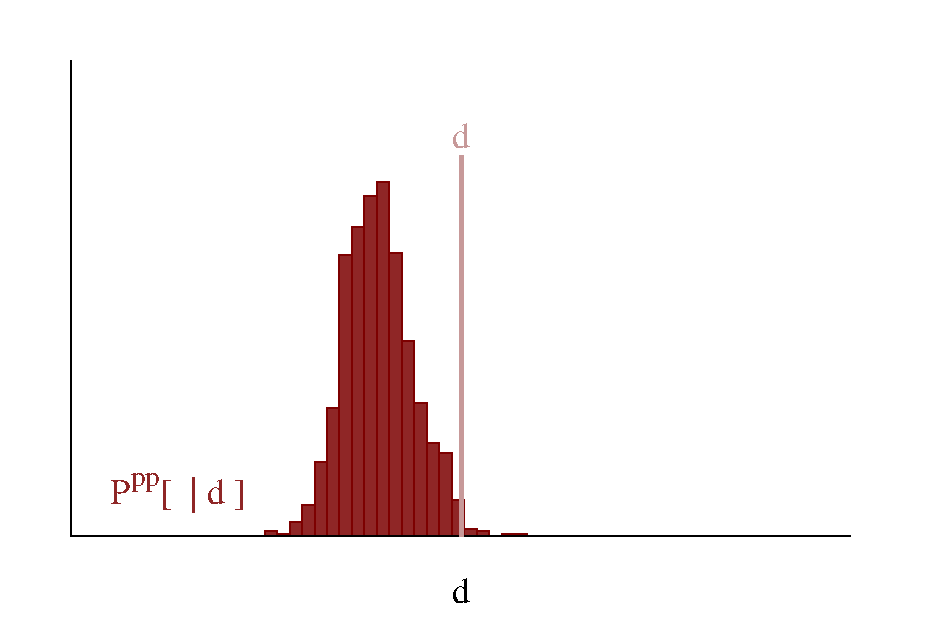
\includegraphics[width=2.75in]{predictive_misfit1.eps} }
\subfigure[]{ 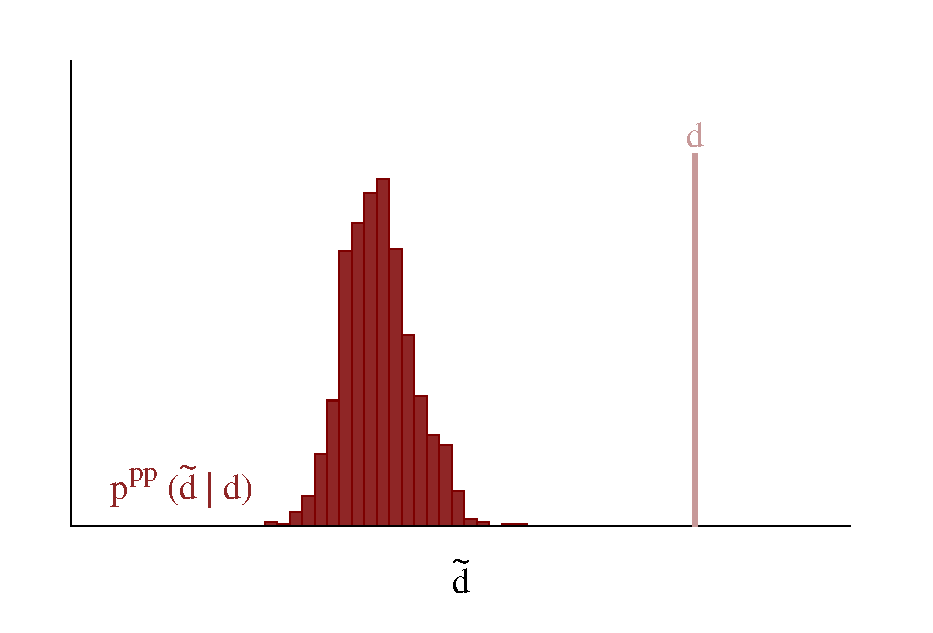
\includegraphics[width=2.75in]{predictive_misfit2.eps} }
\caption{(a) When the measurement, $d$, is consistent with the 
posterior predictive distribution we have no reason to doubt our 
model assumptions, but (b) tension between the measurement and
the posterior predictive distribution indicates that there may be a
problem.  Either the measurement was exceedingly rare or our
model assumptions are insufficient.
}
\label{fig:predictive_misfit}
\end{figure*}

We can also construct a \emph{jackknife posterior predictive
check} by splitting our measurement into two partitions.  Tension
between the marginalized predictive distribution constructed from
one partition and the second partition indicates either an unlikely
measurement or the overfit of the underlying model (Figure
 \ref{fig:predictive_overfit}).

\begin{figure*}
\centering
\subfigure[]{ 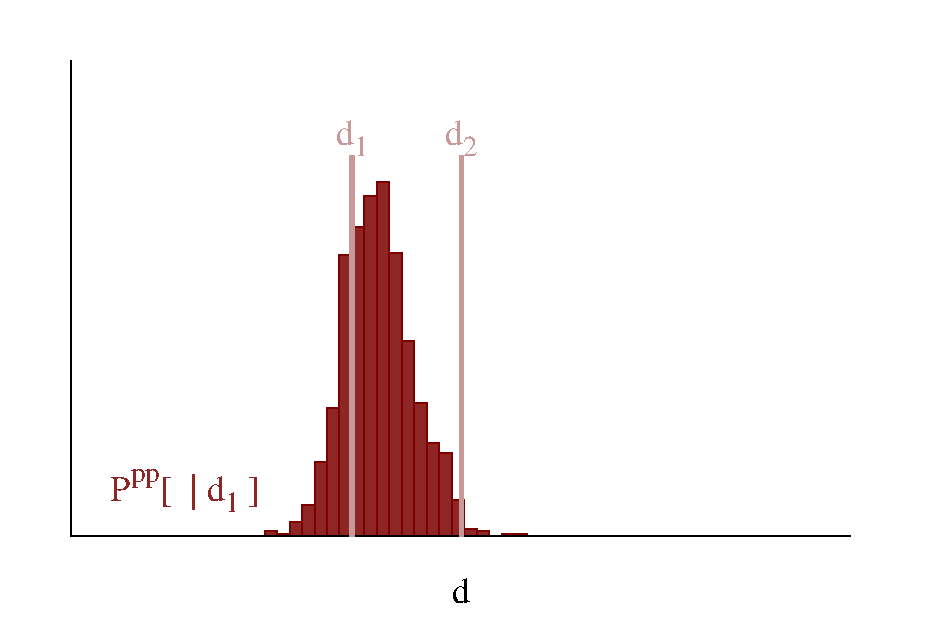
\includegraphics[width=2.75in]{predictive_overfit1.eps} }
\subfigure[]{ 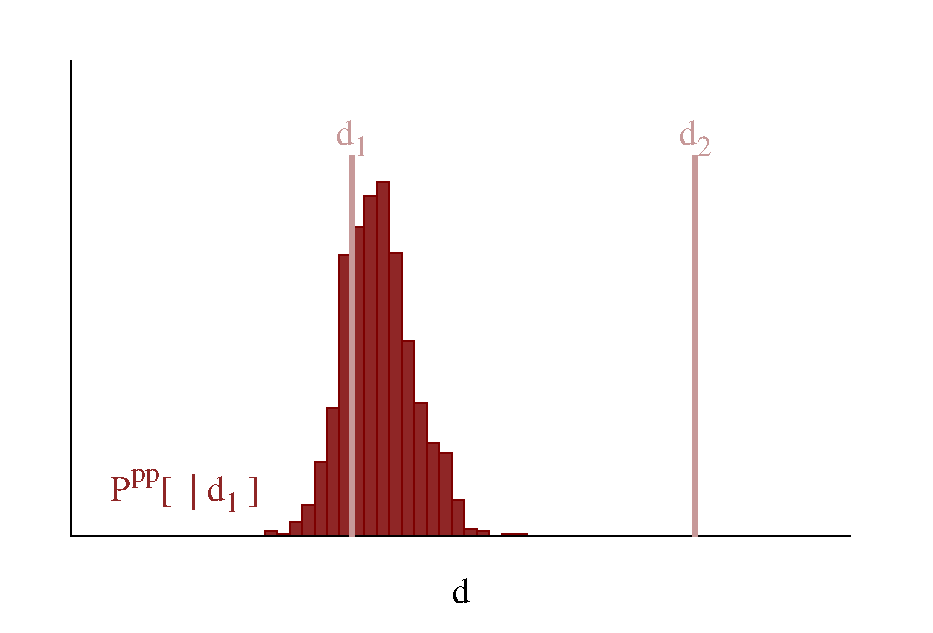
\includegraphics[width=2.75in]{predictive_overfit2.eps} }
\caption{To test for potential overfit we need multiple measurements,
and given only a single measurement this can emulated by splitting
the measurement into two partitions, $d_{1}$ and $d_{2}$.  (a) When 
both measurements are consistent with the posterior predictive 
distribution we have no reason to doubt our model assumptions, but 
(b) tension between the held-out measurement, $d_{2}$ and the 
posterior predictive distribution indicates that the model might be
overfitting to $d_{1}$.  Either the partition generated an exceedingly 
rare measurement or our model assumptions are insufficient.
}
\label{fig:predictive_overfit}
\end{figure*}

As in the general case, these visual predictive checks are not
calibrated and so we cannot discriminate between rare 
measurements and the illegitimacy of our model assumptions.
In practice, however, we can appeal to some implicit baseline
predictive performance to make qualitative judgements as to 
when the tension is strong enough to be suspect.  Suspicion 
then motivates a careful study of the model assumptions that 
manifest in the chosen component of the measurement, and 
potentially the updating of our model into one more capable 
of capturing the intricacies of our data (Figure \ref{fig:model_updating}).

\begin{figure*}
\centering
%
\subfigure[]{
\begin{tikzpicture}[scale=0.225, thick]
  \draw[color=white] (-15, 0) -- (15, 0);

  \fill[mid] (0, 0) ellipse (13 and 7);
  \node at (12, -6) {$\mathcal{P}_{D}$};
  
  \draw[color=dark, dashed] (3, -1) ellipse (6 and 3);
  \node[color=white] at (8.5, -3.5) {$\Theta$};
  
  \fill[color=white] (-7, 3) circle (8pt)
  node[right, color=white] {$\PP_{D}$};
  
  \begin{scope}
    \clip (3, -1) ellipse (6 and 3);
    \foreach \i in {0, 0.05,..., 1} {
      \fill[opacity={exp(-5 * \i*\i)}, dark] (-1.2, 1.2) circle ({2 * \i});      
    }
  \end{scope} 
\end{tikzpicture}
}
%
\subfigure[]{
\begin{tikzpicture}[scale=0.225, thick]
  \draw[color=white] (-15, 0) -- (15, 0);

  \fill[mid] (0, 0) ellipse (13 and 7);
  \node at (12, -6) {$\mathcal{P}_{D}$};
  
  \draw[color=dark, dashed] (1, 0) ellipse (10 and 6);
  \node[color=white] at (8.5, -3.5) {$\Theta$};
  
   \begin{scope}
    \clip (1, 0) ellipse (10 and 6);
    \foreach \i in {0, 0.05,..., 1} {
      \fill[opacity={exp(-5 * \i*\i)}, dark] (-6, 2) circle ({2 * \i});      
    }
  \end{scope}
  
  \fill[color=white] (-7, 3) circle (8pt)
  node[right, color=white] {$\PP_{D}$};
\end{tikzpicture}
}
\caption{Posterior predictive checks are powerful ways to
make qualitative judgements about the validity of our
model assumptions.  For example, if (a) they suggest 
that our model is misfitting the data then (b) we can
update our model to better capture the features of the
data that are being misfit.
}
\label{fig:model_updating}
\end{figure*}

\section{Bayesian Inference in Practice}

Ultimately, implementing Bayesian inference in practice is
surprisingly straightforward.  Using our expertise about a
system we construct a prior that quantifies our initial
assumptions about the system and a likelihood that
quantifies our assumptions about the latent data generating
process itself.  Given these two inputs we can immediately
construct a posterior distribution, and then all inferential
summaries and decisions reduce to computing the 
corresponding expectations.  Although conceptually simple,
neither of these steps is particularly easy.

Building robust models is an immensely challenging tasks
that requires both expertise with a given system and familiarity
with the wealth of potential techniques for constructions priors
and likelihoods.  Many of these techniques are discussed in
the Stan manual (and potentially here someday, too), but here
we'd like to highlight a particularly powerful approach to building
likelihoods: \emph{generative modeling}.  

Generative modeling builds up a likelihood from latent parameters
to the measurement sequentially, as if we were trying to simulate
the data generating process itself.  By considering the forward
model we can naturally incorporate causal structure, such as a 
physical model, measurement variation, and systematic effects,
such as bias and measurement error.  At each stage we model
deterministic or stochastic relationships with conditional probability
distributions until we have constructed the complete likelihood.
The generative nature of these models facilities communication
and helps to identify which features may be most suspect, 
motivating targeted posterior predictive checks and model updates.
\textbf{Constructive example mirroring the motivating example
in the introduction.}

Once we have specified our assumptions and collected our
data, there many options for approximating the resulting
posterior expectations in practice.  We have discussed many
of these here, and there are always more being developed.
Whichever method we end up using, however, we have to
be careful to validate the accuracy of the estimation, lest a 
biased or highly variable estimator spoil the carefully crafted
model.  Such validation is easier in some computational
techniques than others, and sometimes the fastest algorithms
are the most vulnerable to problems.

Although the modeling and computation steps should ideally
be completely decoupled, in practice they will always interact.
More complex models strain the approximation algorithms in
our toolbox, exhausting our computational resources or
compromising the accuracy of the estimators, and in either 
case undermining the robustness of our analysis.  In practice
we often have to iterate, using the success or failure of a
fit to inform the next generation of model.  Provided we do
this deliberately, taking care to validate both the model assumptions 
and fits, we can use Bayesian inference to make powerful
statements about the world around us.

